\section{要求定義}
ユーザがスマートモビリティレジシステムに求める機能と動作をユースケース図を用いて表す。\ref{usecase}には、ユースケース図を示す。そこで、赤枠で囲っている部分が筆者が担当する。
ユースケース図では、ユーザがスマートモビリティレジシステムに対して動作を行った際に、システムがどのような振る舞いをするかを示す。ユーザは通常の買い物のように、カートに商品を出し入れすることができる。このときカート(RaspberryPi)が商品に関するデータを集める。解析システムでは、商品情報の特定とカゴDBへの操作を行う。解析システムはサーバで動作する。カゴDBは、カート内にある商品情報を管理し、最終的な決済システムで利用される。ユーザがカートを返却すると、決済システムが動作する。決済システムは、顧客の口座(プリペイドカードや電子マネー口座)からカート内の商品合計金額を引く処理を行う。

\begin{figure}[htbp]
\centering
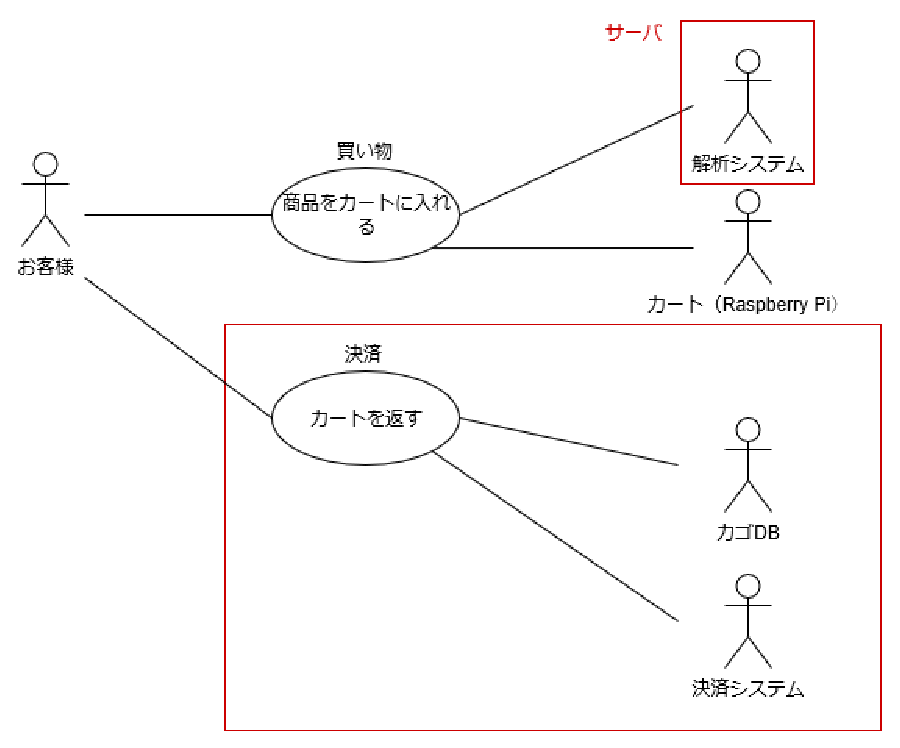
\includegraphics[width=12cm]{./pic/usecase_saishu.eps}
\caption{ユースケース図}
\label{usecase}
\end{figure}

次に、ユースケース図を基にスマートモビリティレジシステムのシナリオを以下の表\ref{scenario}に示す。
\begin{table}[htb]
\begin{center}
\caption{スマートモビリティレジシステムのシナリオ}
\begin{tabular}{|l|c|} \hline
 & シナリオ \\ \hline \hline
買い物 & 商品を置く→バーコード認識→商品DB追加・削除→結果通知 \\
決済 & ユーザが退店する→決済を行う \\ \hline
\end{tabular}
\label{scenario}
\end{center}
\end{table}

次に、要求定義を満たす機能テスト項目を以下の表\ref{integrated_test}を示す。

\begin{table}[htbp]
\centering
\caption{総合テスト項目}
\includegraphics[width=15cm]{./pic/integrated_test.eps}
\label{integrated_test}
\end{table}